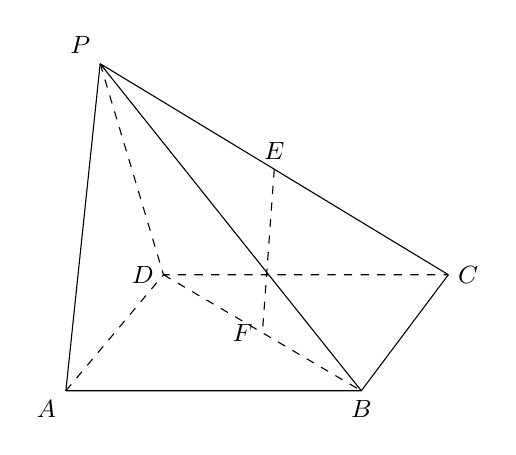
\begin{tikzpicture}[scale=.67, every node/.style={font=\small}]
  \coordinate (A) at (0,0);
  \coordinate (B) at (5.6,0);
  \coordinate (C) at (7.25,2.2);
  \coordinate (D) at (1.85,2.2);
  \coordinate (P) at (.65,6.2);
  \coordinate (E) at (3.95,4.2);
  \coordinate (F) at (3.725,1.1);

  \draw (A)--(B)--(C) (P)--(A) (P)--(B) (P)--(C);
  \draw[dashed] (A)--(D)--(C) (P)--(D) (D)--(F)--(B) (E)--(F);

  \node[below left]  at (A) {$A$};
  \node[below]       at (B) {$B$};
  \node[right]       at (C) {$C$};
  \node[left]        at (D) {$D$};
  \node[above left]  at (P) {$P$};
  \node[above]       at (E) {$E$};
  \node[left]        at (F) {$F$};
\end{tikzpicture}
